\section{Processi di supporto}
\subsection{Processo di documentazione}
In questa sezione verranno descritti tutti i metodi ed i procedimenti utilizzati per registrare le informazioni prodotte dal ciclo di vita di un processo o di una attività.

\subsubsection{Descrizione}
Tratteremo di seguito tutte le convenzioni adottate dal \termine{team} per produrre i documenti dove registrare le informazioni sopra dette, e tutti i metodi per standardizzare la loro  stesura, verifica e approvazione. \\
I documenti vengono classificati come:
\begin{itemize}
  \item \textit{Interni} se il loro utilizzo rimane interno al \termine{team}.
  \item \textit{Esterni}: se la loro distribuzione avviene anche alle componenti esterne al gruppo, come ad esempio il committente e/o il proponente.
\end{itemize}

I documenti \textit{approvati} dal \textit{\Pm} devono avere un nome strutturato nel seguente modo:
\begin{itemize}
  \item La prima lettera del documento deve essere maiuscola.
  \item Il nome non deve contenere spazi e deve essere scritto in \termine{camel case} per identificare. 
  \item La versione del documento deve essere indicata nella parte finale del nome in forma numerica
  \begin{center}
  \textit{NomeDelDocumento\_v.1.0.0}
  \end{center}\
\end{itemize}
Inoltre nel documento deve essere specificato il suo scopo (facilmente comprensibile dal suo titolo) e  nel diario delle modifiche dovranno essere elencati i soggetti che hanno preso parte alla stesura, modifica, verifica e approvazione del documento stesso.

\subsubsection{Strumenti}
Per la stesura dell'intera documentazione è stato scelto di utilizzare \textit{\termine{LaTeX}} in quanto questo \termine{linguaggio di markup} permette di avere uno
standard comune ed evitare possibili conflitti e incompatibilità derivanti
dall'utilizzo di software differente.

\subsubsection{Struttura del documento}
\paragraph{Prima pagina}
Ogni documento deve avere nella prima pagina le seguenti informazioni:
\begin{itemize}
  \item Nome del gruppo.
  \item Logo del progetto.
  \item Nome del progetto.
  \item Nome del documento.
  \item Versione del documento.
  \item Data di creazione del documento.
  \item Data di ultima modifica del documento.
  \item Stato del documento.
  \item Nome e cognome del redattore del documento.
  \item Nome e cognome del verificatore del documento.
  \item Nome e cognome del responsabile approvatore del documento.
  \item Uso del documento.
  %\item Lista di distribuzione del documento.
  \item Destinatari del documento.
  \item Un sommario contenente una breve descrizione del documento.
\end{itemize}

\paragraph{Diario delle modifiche}
La seconda pagina di ogni documento deve contenere il diario delle modifiche. In questa tabella vengono inserite tutte le modifiche effettuate dai vari redattori del documento. Ogni
riga della tabella deve contenere le seguenti informazioni:
\begin{itemize}
  \item \textbf{Descrizione - Motivazione}: descrizione della modifica apportata. Dopo il '-' deve essere inserita invece la motivazione della modifica.
  \item \textbf{Autore e Ruolo}: autore della modifica e ruolo che esso ricopre.
  \item \textbf{Data}: data della modifica apportata.
  \item \textbf{Versione}: versione del documento dopo la modifica.
\end{itemize}

\paragraph{Indice}
In ogni documento, dopo il diario delle modifiche, deve essere presente un
indice di tutte le sezioni. In presenza di tabelle e/o immagini queste devono
essere indicate con i relativi codici identificati.

\paragraph{Formattazione generale delle pagine}
La formattazione della pagina, oltre al contenuto, prevede un'intestazione e un
piè di pagina. \\
L'intestazione della pagina contiene:
\begin{itemize}
  \item Nome del progetto.
  \item Nome del documento.
  \item Logo del gruppo.
\end{itemize}
Il piè di pagina contiene:
\begin{itemize}
  \item Il nome del gruppo.
  \item Email del gruppo.
  \item Numero della pagina corrente.
\end{itemize}

\subsubsection{Norme tipografiche}
Le seguenti norme tipografiche indicano i criteri riguardanti l'ortografia e la tipografia di tutti i documenti.

\paragraph{Stili di testo}
\begin{itemize}
  \item \textbf{Grassetto}: Il grassetto deve essere utilizzato per evidenziare parole
  particolarmente importanti, negli elenchi puntati o nelle frasi.
  \item \textbf{Corsivo}: Il corsivo deve essere utilizzato nelle seguenti
  situazioni:
  \begin{itemize}
    \item Ruoli: ogni riferimento a ruoli di progetto va scritto in corsivo.
    \item Documenti: ogni riferimento a un documento va scritto in corsivo.
    \item Stati del documento: ogni stato del documento va scritto in corsivo.
    \item Citazioni: ogni citazione va scritta in corsivo.
    \item Glossario: ogni parola presente nel glossario, oltre ad avere un pedice, deve
    essere scritta in corsivo.
  \end{itemize}
\end{itemize}

\paragraph{Composizione del testo}
\begin{itemize}
   \item \textbf{Glossario}: il pedice \termine{} verrà utilizzato in corrispondenza di vocaboli presenti nel \textit{\glossario}.
\end{itemize}

\paragraph{Formati}
\begin{itemize}
   \item \textbf{Date}: le date presenti nei documenti devono seguire lo standard seguente:
   \begin{center}
     GG-MM-AA
   \end{center}
   dove:
   \begin{itemize}
   		\item GG rappresenta il giorno.
     	\item MM rappresenta il mese.
     	\item AA rappresenta l'anno.
   \end{itemize}
   \item \textbf{Ore}: le ore presenti nei documenti devono seguire lo standard seguente (a 24 ore):
   \begin{center}
     hh:mm
   \end{center}
   dove:
   \begin{itemize}
     \item hh: rappresentano le ore.
     \item mm: rappresentano i minuti.
   \end{itemize}
   \item \textbf{Nome del documento}: per riferirsi al nome del documento si
   dovrà utilizzare il comando \termine{LaTeX} \\ \verb|\Nome del documento| garantendo in questo modo la corretta sintassi.
   \item \textbf{Nome del gruppo}: per riferirsi al nome del gruppo si dovrà
   utilizzare il comando \termine{LaTeX} \verb|\gruppo| garantendo in questo modo la corretta sintassi.
   \item \textbf{Nome del progetto}: per riferirsi al nome del progetto si dovrà
   utilizzare il comando \termine{LaTeX} \verb|\progetto| garantendo in questo modo la corretta sintassi.
   \item \textbf{Link sito del gruppo}: per riferirsi al link del sito del gruppo si dovrà
   utilizzare il comando \termine{LaTeX} \verb|\gruppoLink| garantendo in questo modo la corretta sintassi.
   \item \textbf{Email del gruppo}: per riferirsi all'indirizzo email del gruppo si dovrà
   utilizzare il comando \termine{LaTeX} \verb|\email| garantendo in questo modo la corretta sintassi.
   \item \textbf{Nome del proponente}: per riferirsi al nome del proponente, ovvero \proponente, si dovrà
   utilizzare il comando \termine{LaTeX}  \verb|\proponente| garantendo in questo modo la corretta
   sintassi.
\end{itemize}

\subsubsection{Componenti grafiche}
\paragraph{Tabelle}
Tutte le tabelle presenti all'interno del documento devono avere una didascalia
ed un codice identificativo univoco.

\paragraph{Immagini}
Le immagini inserite nel documento devono essere in formato \termine{PNG}.

\subsubsection{Composizione email}
Di seguito vengono descritte le norme da applicare nella composizione delle email.

\paragraph{Destinatario}
\begin{itemize}
  \item Interno: l'indirizzo da utilizzare è \email.
  \item Esterno: l'indirizzo del destinatario varia a seconda si tratti del Prof. Tullio Vardanega \\ (\link{tullio.vardanega@math.unipd.it}), del Prof. Riccardo Cardin (\link{rcardin@math.unipd.it}) o i proponenti del progetto.
\end{itemize}

\paragraph{Mittente}
\begin{itemize}
  \item Interno: l'indirizzo è di colui che scrive l'email.
  \item Esterno: l'indirizzo da utilizzare è \email e può usarlo unicamente il \Pm.
\end{itemize}

\paragraph{Oggetto}
L'oggetto della mail deve essere esplicito, comprensibile e conciso in modo da rendere
immediato il riconoscimento del contenuto.

\paragraph{Corpo}
Il testo del corpo della mail deve essere esaustivo. All'interno del
testo ci si potrà riferire a un ruolo preciso all'interno del team o a un destinatario univoco.

\paragraph{Allegati}
È sconsigliato l'invio di allegati tramite mail in quanto è preferibile condividere file all'interno del gruppo tramite strumenti più adatti, come \termine{Google Drive}.

\subsubsection{Produzione di documenti}
I documenti prodotti come sopra detto verranno innanzitutto creati con il linguaggio di markup \termine{LaTeX}, e successivamente salvati in formato \termine{PDF}. I tipi di documento prodotti sono i seguenti.

\paragraph{\SdF}
Questo documento riporta le motivazioni che hanno portato l'intero
\termine{team} all'accettazione dello sviluppo del progetto scelto. E' un documento interno e la lista di distribuzione riguarda i committenti.

\paragraph{\NdP}
Questo documento riporta le convenzioni, strumenti e
norme che il \termine{team} ha scelto di adottare durante  lo sviluppo del progetto. Questo
documento è interno e la lista di distribuzione riguarda i committenti.

\paragraph{\PdP}
Questo documento descrive come il \termine{team} gestisce le risorse, temporali e umane, a disposizione e come sono stati valutati e trattati i rischi. Questo documento è esterno e la lista di distribuzione comprende sia i committenti che i proponenti.

\paragraph{\PdQ}
Questo documento descrive in che maniera l'intero \termine{team} cerca di soddisfare gli obiettivi di qualità del progetto. Questo documento è esterno e la lista di distribuzione comprende sia i committenti che i proponenti.

\paragraph{\AdR}
Questo documento dà una visione dell'insieme dei casi d'uso del progetto e dei requisiti derivati da essi. Contiene inoltre i diagrammi delle attività di interazione tra utente e sistema sviluppato e i servizi che il progetto, una volta concluso, andrà ad erogare. È un documento esterno e la lista di distribuzione comprende committenti che i proponenti.

\paragraph{\SdF}
L'intento del suddetto documento è dare una visione generale del prodotto e delle sue richieste. Più nello specifico verrà mostrata una progettazione ad alto livello, basata su diagrammi dei \termine{package} per la descrizione delle componenti, diagrammi di sequenza per descrivere gli scenari d'uso e diagrammi di attività. Verranno inoltre elencati i software che saranno utilizzati per la realizzazione del progetto. Questo è un documento esterno e la sua lista di distribuzione comprende  sia i committenti che i proponenti.

\paragraph{\DDP}
L'intento di tale documento è fornire una progettazione dettagliata del
prodotto. In esso verranno forniti tutti i suoi dettagli implementativi, fondamentali in fase di codifica, che comprenderanno diagrammi \termine{UML} delle classi e i relativi metodi. Questo è un documento esterno e la sua lista di distribuzione comprende  sia i committenti che i proponenti.

\paragraph{\Gl}
Questo documento viene prodotto al fine di dare una spiegazione dettagliata dei termini tecnici e degli acronimi utilizzati nell'intera documentazione. La sua lista di distribuzione comprende i committenti che i proponenti ed è quindi un documento esterno.

\paragraph{\MU}
Questo documento fornisce all'utente una guida delle funzionalità e dei servizi offerti dal prodotto. Essendo una guida destinata all'utente è un documento esterno e la sua lista di distribuzione comprende i sopracitati utenti. \\

\textbf{N.B.} Come definito all'interno del \textit{Verbale esterno del 03 maggio 2017}, nel punto \textit{VE10.1}, il \MU\ realizzato per \progettoShort\ potrà non essere redatto seguendo le indicazioni sopra descritte previste per gli altri documenti, a seguito di quanto deciso in concordanza con il proponente \RB.

\paragraph{Verbale}
Questo documento ha lo scopo di riassumere in modo formale le discussioni effettuate e le decisioni prese durante le riunioni. I verbali, come i documenti, sono classificati in:
\textbf{interni} ed \textbf{esterni}. In particolare i verbali esterni, essendo ufficiali, devono essere redatti dal \Pm. \\
Ogni verbale dovrà essere denominato nel seguente modo:
\begin{center}
  \textit{{Verbale}\_{Numero del verbale}\_{Data del verbale}}
\end{center}
dove:
\begin{itemize}
  \item \textbf{Numero del verbale} è numero identificativo univoco del verbale.
  \item \textbf{Data del verbale} identifica la data nella quale si è svolta la
  riunione corrispondente al verbale. Il formato è il seguente :
  \begin{center}
  YYYY-MM-DD
  \end{center}
\end{itemize}
Cosi come per i documenti anche per i verbali si è cercato di standardizzare la loro struttura, e pertanto la  parte introduttiva deve essere correlata con le seguenti informazioni:
\begin{itemize}
  \item \textbf{Data incontro}: data in cui si è svolta la riunione.
  \item \textbf{Ora inizio incontro}: orario di inizio della riunione.
  \item \textbf{Ora termine incontro}: orario di terminazione della riunione.
  \item \textbf{Luogo incontro}: luogo in cui si è svolta la riunione.
  \item \textbf{Durata}: durata della riunione.
  \item \textbf{Oggetto}: argomento della riunione.
  \item \textbf{Segretario}: nome e cognome del membro incaricato a redigere il
  verbale.
  \item \textbf{Partecipanti}: nome e cognome di tutti i membri partecipanti alla riunione.
  
\end{itemize}
Verrà poi descritto sinteticamente l'\textit{ordine del giorno} dove verranno elencati tutti gli argomenti di cui si è discusso nel verbale.
Infine verrà descritta la decisione presa, essa sarà tracciata secondo il seguente schema: 
\begin{center}
\textit{V(tipo)(codice)}
\end{center}
dove:
\begin{itemize}
\item \textbf{tipo}: I se interno E se esterno;
\item \textbf{codice}: NumeroVerbale.IndiceDecisione \\ \\ dove:
\begin{itemize}
\item \textbf{NumeroVerbale}: descrive il verbale in cui la decisione è stata presa.
\item \textbf{IndiceDecisione}: E' un indice di tipo gerarchico dove si indicizza la decisone, ad esempio decisione 5, sottodecisione 5.3 .
\end{itemize}
\end{itemize}

\subsubsection{Ciclo di vita di un documento}
 I documenti possono avere 3 stati diversi:
\begin{itemize}
  \item Documenti \textbf{in lavorazione}.
  \item Documenti \textbf{da verificare}.
  \item Documenti \textbf{approvati}.
\end{itemize}
I documenti \textbf{in lavorazione} sono quelli in fase di stesura da parte del relativo redattore. Ultimata la loro realizzazione questi documenti vengono segnati come \textbf{da verificare} e passano in mano al relativo \Ver. Infine i documenti \textbf{verificati} vengono consegnati al \Pm che avrà il compito di approvarli definitivamente. Nella figura 1.0 è rappresentato lo schema del ciclo di vita di un documento

\subsubsection{Versionamento}
Ogni documento prodotto deve essere identificato, oltre che dal nome, dal numero
di versione nel seguente modo:
\begin{center}
  \_v.X.Y.Z
\end{center}
dove:

\begin{itemize}
  \item \textbf{X}: indica il numero di uscite formali del documento e viene incrementato in seguito all'approvazione finale da parte del \textit{\Pm}.
  L'incremento dell'indice \textbf{X} comporta l'azzeramento degli indici
  \textbf{Y} e \textbf{Z}.
  \item \textbf{Y}: indica il numero crescente delle verifiche. L'incremento viene 	eseguito dal \textit{\Ver} e comporta l'azzeramento dell'indice \textbf{Z}.
  \item \textbf{Z}: indica il numero di modifiche minori apportate al documento
  prima della sua verifica e viene aumentato ad ogni modifica apportata.
  \end{itemize}
A ogni modifica del documento anche il nome del file fisico deve essere
modificato, seguendo lo stesso schema precedentemente proposto:
\begin{center}
  nomeDocumento\_v.X.Y.Z.pdf
\end{center}

\subsubsection{Strumenti}
\paragraph{LaTeX}
Lo strumento che il \termine{team} ha scelto per la stesura e la manutenzione di tutti i documenti è \termine{LaTeX}. Le ragioni che hanno portato a questa scelta sono:
\begin{itemize}
\item La disponibilità di mezzi per l'automazione della maggior parte della composizione tipografica.
\item La possibilità di definire \termine{template} dei documenti da stilare.
\item La possibilità di utilizzarlo gratuitamente e ovunque grazie alla sua licenza \termine{open source}.
\item La possibilità di suddivisione del documento in file separati al fine di facilitare il lavoro in gruppo.
\item La disponibilità di strumenti di controllo ortografico per minimizzare i possibili errori tipografici.
\item La facilità d'uso e di configurazione.
\item La possibilità di conversione del testo scritto in file \termine{PDF}.
\item Gli editor usati usati per \termine{LaTeX} son \termine{Texmaker} su MacOS e Windows 10 e \termine{Gummi}.
\item Per creare il glossario è stato implementato un script automatico in \termine{python} che attraverso un file json contenente i vocaboli e le loro definizioni genera il glossario. Per far funzionare correttamente lo script è necessario che i redattori del documento marchino con il rispettivo comando "$\backslash$termine" gli elementi da inserire nel glossario.
\end{itemize}

\subsection{Processo di configurazione}

\label{figura 1.0}
\begin{figure}[ht]
	\centering
	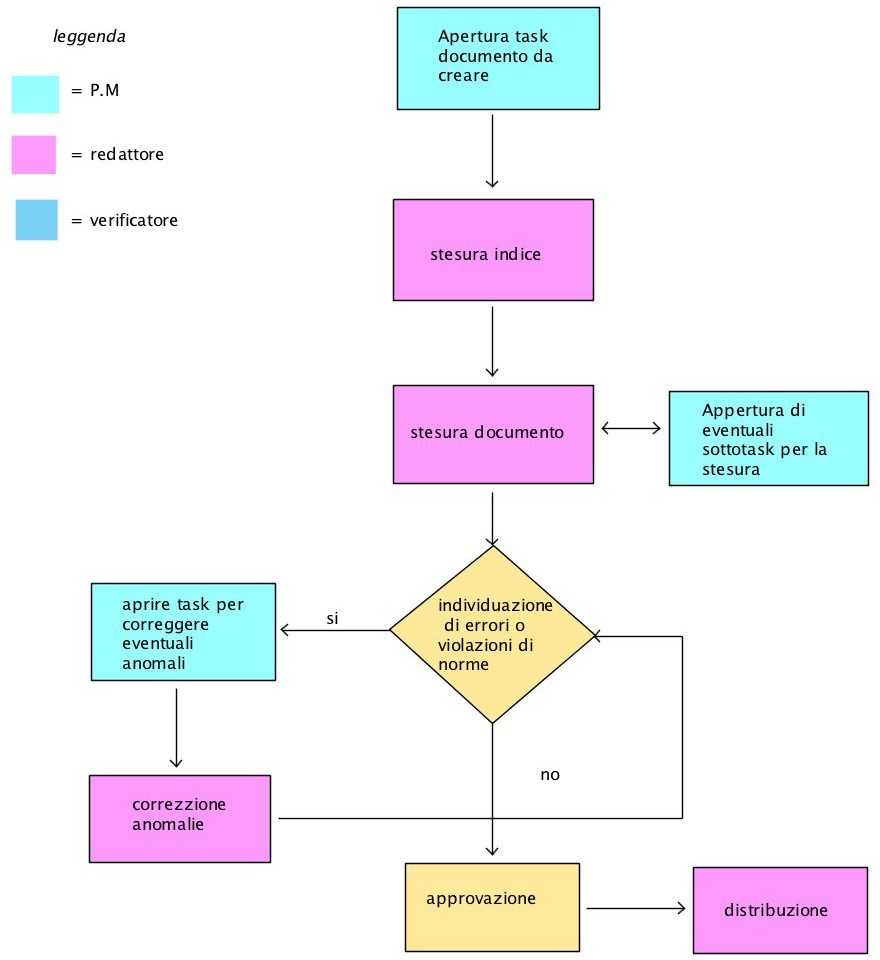
\includegraphics[scale=0.8]{ciclo_di_vita.jpg}
	\caption{Ciclo di vita di un documento}
\end{figure}

\subsubsection{Scrittura dei documenti}
È stato steso un piano generale per la stesura dei documenti, in modo da definire le varie parti da stendere e come queste interagiscano tra loro.
Per ogni documento verranno assegnati diversi task (descritti nella Figura 1) ai diversi componenti del \termine{team}, ciascuno con dei propri o. Per assegnare i task e determinare le date di ciascuna \termine{milestone} è stato usato un strumento di pianificazione, \termine{Wrike}, come descritto in dettaglio nella sezione 1.3.4 di questo documento.

\subsubsection{Gestione delle configurazioni}
Per controllare le versioni e le modifiche applicate al software viene utilizzata una \termine{repository} su \termine{GitHub}. All'interno di essa ogni partecipante può verificare l'integrità e la correttezza delle modifiche applicate. Inoltre, per ogni modifica effettuata, viene fatto un \termine{commit} con lo scopo di tenere traccia di ogni variazione effettuata nel ciclo di sviluppo. Ogni volta che deve venire accettata una modifica bisogna effettuare un 	\termine{push} del software modificato che risiede nella \termine{repository} (con il relativo \termine{commit}), e prima di essere accettato saranno presenti dei testi di integrazione automatici sviluppati con i framework \termine{SonarQube} e \termine{Jenkins} implementati nella \termine{repository} di \termine{GitHub} tramite \termine{webhook}.

\subsubsection{Strumenti}

\paragraph{GitHub}
Gli strumenti per il versionamento rendono possibile lo sviluppo del software in maniera controllata e quantificabile. È stato quindi deciso di creare una \termine{repository} che ospiterà documenti digitali e manuali, oltre che al codice sorgente del software, rendendo possibile il tracciamento della loro evoluzione. \\
Il software di versionamento scelto è \termine{Git} perché presenta molti più aspetti positivi rispetto ad altri sistemi di versionamento centralizzati. \termine{Git} permette ai membri del \termine{team} di copiare la \termine{repository} in locale, lavorandoci anche in assenza di connessione, per poi successivamente caricare nuovamente su di essa i file modificati. \\
Il servizio scelto per l'\termine{hosting} delle \termine{repository} contenenti rispettivamente i documenti, il codice sorgente dell'\termine{SDK} e il codice sorgente della applicazione \termine{demo} è \termine{GitHub} e la loro struttura base è la seguente:
\begin{itemize}
  \item \termine{Repository} dei documenti
  	\begin{itemize}
  		\item RR
			\begin{itemize}
				\item Interni
				\item Esterni
			\end{itemize}
  		\item RQ
  			\begin{itemize}
				\item Interni
				\item Esterni
			\end{itemize}
  		\item RP
  			\begin{itemize}
				\item Interni
				\item Esterni
			\end{itemize}
  		\item RA
  			\begin{itemize}
				\item Interni
				\item Esterni
			\end{itemize}
  		\item \termine{Template}   			\begin{itemize}
  				\item Firme
  			\end{itemize}
  	\end{itemize}
  	\item \termine{Repository} del codice sorgente dell'\termine{SDK}
  		\begin{itemize}
  			\item Codice sorgente dell'\termine{SDK}
  		\end{itemize}
  	\item \termine{Repository} del codice sorgente dell'applicazione \termine{demo}
  		\begin{itemize}
  			\item Codice sorgente dell'applicazione \termine{demo}
  		\end{itemize}
  	
\end{itemize}

\subparagraph{Regole per il push}
Il team ha standardizzato i \termine{push} da effettuare nella \termine{Repository} contenente i documenti. Dovrà essere specificato il documento (documenti se più di uno) modificati/creati in quel particolare commit. Non è ancora stato definito un metodo unico per i \termine{push} effettuati nella codifica del codice. Esso verrà definito prima dell'inizio dell'attività di codifica.

\paragraph{Git}
Come sistema di controllo di versionamento la scelta è ricaduta obbligatoriamente su \termine{Git} avendo scelto GitHub come host.

\newpage

\subsection{Processo di garanzia di qualità del prodotto}
Per garantire la qualità del prodotto vengono adottato varie metodologie tra le quali ritroviamo i processi di verifica e di validazione successivamente illustrati. \\
Nel caso in cui i task assegnati al team non siano soddisfatti per eventuali problematiche, questi devono essere riportati nella lista di problemi menzionata nel \textit{processo di soluzione di problemi}. \\
Un ulteriore garanzia di qualità è data dall'assicurarsi che i requisiti principali del progetto siano soddisfatti alla fine dello sviluppo del software. Ci si può assicurare di questo attraverso una documentazione valida ed un incontro con i committenti ed i proponenti che dovranno accertarsi della validità del prodotto finale. \\
Infine per stabilire in maniera quantitativa la qualità ottenuta abbiamo individuato delle metriche che andremo ora a esplicitare, indicando i range accettabili e quelli ottimali. Il loro valore effettivo è invece indicato nel Piano di qualifica.
Le metriche individuate sono state suddivise in
\begin{itemize}
	\item\textbf{\termine{Qualità funzionale}}.
	\item\textbf{\termine{Qualità di affidabilità}}.
	\item\textbf{\termine{Qualità di usabilità}}.
	\item\textbf{\termine{Qualità di efficienza}}.
	\item\textbf{\termine{Qualità di manutenibilità}}.
\end{itemize}

\subsubsection{Qualità funzionale}

\paragraph{Completezza dell'implementazione funzionale}
Indica la percentuale di requisiti funzionali coperti dall'implementazione.
\begin{itemize}
	\item \textbf{Misurazione}: 
		$$C=\left(1-\mathlarger{\frac{N_{FM}}{N_{FI}}}\right) \cdot 100$$ 
	dove $N_{FM}$ è il numero di funzionalità mancanti nell'implementazione e $N_{FI}$ è il numero di funzionalità individuate nell'attività di analisi.
\end{itemize}

\paragraph{Accuratezza rispetto alle attese}
Indica la percentuale di risultati concordi alle attese.
\begin{itemize}
	\item \textbf{Misurazione}: 
		$$A=\left(1-\mathlarger{\frac{N_{RD}}{N_{TE}}}\right) \cdot 100$$
	dove $N_{RD}$ è il numero di test che producono risultati discordanti rispetto alle attese e $N_{TE}$ è il numero di test-case eseguiti.
\end{itemize}

\subsubsection{Qualità di affidabilità}
\paragraph{Densità di \textit{failure}}
Indica la percentuale di operazioni di testing che si sono concluse in fallimenti.

\begin{itemize}
	\item \textbf{Misurazione}: 
		$$F=\mathlarger{\frac{N_{FR}}{N_{TE}}} \cdot 100$$
	dove $N_{FR}$ è il numero di fallimenti rilevati durante l'attività di testing e $N_{TE}$ è il numero di test-case eseguiti.
\end{itemize}

\paragraph{Blocco di operazioni non corrette}
Indica la percentuale di funzionalità in grado di gestire correttamente i \textit{fault} che potrebbero verificarsi.
\begin{itemize}
	\item \textbf{Misurazione}: 
		$$B=\mathlarger{\frac{N_{FE}}{N_{ON}}} \cdot 100$$
	dove $N_{FE}$ è il numero di \textit{failure} evitati durante i test effettuati e $N_{ON}$ è il numero di test-case eseguiti che prevedono l'esecuzione di operazioni non corrette, causa di possibili \textit{failure}.
\end{itemize}

\subsubsection{Qualità di efficienza}

\paragraph{Tempo di risposta}
Indica il periodo temporale medio che intercorre fra la richiesta al software di una determinata funzionalità e la restituzione del risultato all'utente.
\begin{itemize}
	\item \textbf{Misurazione}: 
		$$T_{RISP} = \mathlarger{\frac{\sum_{i=1}^{n} T_{i}}{n}}$$ 
	con $T_{RISP}$ misurato in secondi, e dove $T_{i}$ è il tempo intercorso fra la richiesta $i$ di una funzionalità ed il completamento delle operazioni necessarie a restituire un risultato a tale richiesta.
\end{itemize}
\subsubsection{Qualità di manutenibilità}

\paragraph{Capacità di analisi di \textit{failure}}
Indica la percentuale di \textit{failure} registrate delle quali sono state individuate le cause.
\begin{itemize}
	\item \textbf{Misurazione}: 
		$$I=\mathlarger{\frac{N_{FI}}{N_{FR}}} \cdot 100$$
	dove $N_{FI}$ è il numero di \textit{failure} delle quali sono state individuate le cause e $N_{FR}$ è il numero di \textit{failure} rilevate.
\end{itemize}

\paragraph{Impatto delle modifiche}
Indica la percentuale di modifiche effettuate in risposta a \textit{failure} che hanno portato all'introduzione di nuove \textit{failure} in altre componenti del sistema.
\begin{itemize}
	\item \textbf{Misurazione}: 
		$$I=\mathlarger{\frac{N_{FRF}}{N_{FR}}} \cdot 100$$
	dove $N_{FRF}$ è il numero di \textit{failure} risolte con l'introduzione di nuove \textit{failure} e $N_{FR}$ è il numero di \textit{failure} risolte.
\end{itemize}


			
\subsection{Processo di verifica}
\subsubsection{Descrizione}
Il processo di verifica ha il compito di controllare che ogni documento e software prodotto dal \termine{team} non presenti eventuali anomalie o errori e che esso rispecchi quanto previsto dai requisiti ad esso associati. In generale esistono due tipi di analisi nel mondo informatico, l'analisi statica e quella dinamica che andremo successivamente a elencare. Per rendere quantificabile il processo di verifica abbiamo scelto anche delle metriche per misurare la qualità dei processi.

\paragraph{Metriche per la pianificazione}
Qualsiasi eventuale valore negativo ottenuto dalle  metriche: Schedule Variance o/e Budget Variance dovrà essere  compensato entro la fine dell'attività di progetto modficando e revisionando in modo coerente il \PdP, in quanto non è possbile eccedere le ore di lavoro finali e il budget finale indicato nella pianificazione.
						
\subparagraph{Schedule Variance}
Indica se si è in linea, in anticipo o in ritardo rispetto la pianificazione temporale prevista dal Piano di Progetto.
Per calcolare questa metrica utilizziamo la seguente formuala: SV = BCWP −BCWS, dove BCWP sono le attività completate ad un certo momento e BCWS
le attività che, secondo la pianificazione, dovrebbero essere state completate a quel momento.
Il range di accettazione per questa metrica è un valore superiore o uguale a zero in questo modo ci si assicura di non avere accumulato eventuali ritardi per la consegna.

\subparagraph{Budget Variance}
Indica se alla data corrente si è speso di più o di meno rispetto a quanto pianificato.
Per calcolare questa metrica utilizziamo la seguente forumal: BV = BCWS − ACWP , dove BCWS è il costo pianificato per realizzare le attività di progetto
alla data corrente e ACWP è il costo effettivamente sostenuto alla data corrente.
Il range di accettazione per questa metrica è un valore superiore o ugale a zero, segnale che i costi sono stati preventivati in maniera corretta e non si esce dal budget prefeissato all'inizio


\subparagraph{Ottimalità delle misurazioni}
Questa metrica misura quante metriche misurate sono ottimali e assicura che almeno una buona quantita lo siano.
\textbf{Misurazione:} 
\begin{displaymath}
{\text{Misurazioni Ottimali}}\over{\text{Misurazioni Ottimali} + \text{Misurazioni Accettabili}}
\end{displaymath} 
Il valore di accettazione è pari a 0.3 mentre il valore ottimale è 0.4 questo per garantire l'ottimo range per almeno un numero cospicuo di metriche così da aumentare la qualità del software.

\subparagraph{Requisiti obbligatori soddisfatti}
Indica il numero di requisiti obbligatori ottenuti dall'attività di analisi.
\begin{itemize}
\item \textbf{Misurazione}: 
		$$C=\left(1-\mathlarger{\frac{N_{FM}}{N_{FI}}}\right) \cdot 100$$ 
\end{itemize}
dove $N_{FM}$ è il numero di funzionalità mancanti nell'implementazione e $N_{FI}$ è il numero di funzionalità individuate nell'attività di analisi. 



\paragraph{Metriche per i documenti}
\subparagraph{indice di Gulpease}
L'indice Gulpease rispetto ad altri indici di leggibilità possiede il vantaggio di utilizzare la lunghezza delle parole in lettere anziché in sillabe, semplificando il calcolo dell'indice stesso. Esso considera due variabili linguistiche:
\begin{itemize}
\item La lunghezza della parola.
\item La lunghezza della frase rispetto al numero delle lettere.
\end{itemize}

I valori dell'indice sono compresi tra 0 e 100, dove il valore 100 indica la leggibilità più alta e 0 la leggibilità più bassa.

\paragraph{Metriche per la progettazione dell'architettura di sistema}

\subparagraph{Livello di instabilità}
Per comprendere questa metrica è necessario dare una semplice spiegazione di \termine{accoppiamento afferente} e di \termine{accoppiamento efferente}.
\begin{itemize}
\item
\textbf{Accoppiamento afferente}: indica il numero di classi esterne ad un \termine{package} che dipendono da classi interne ad esso.
Un alto valore implica un alto grado di dipendenza del resto del software dal \termine{package}. Un valore eccessivamente basso, invece, potrebbe evidenziare che un \termine{package} fornisce poche funzionalità.
\item
\textbf{Accoppiamento efferente}: indica il numero di classi interne al \termine{package} che dipendono da classi esterne ad esso.
Mantenendo il valore di tale indice basso è possibile garantire funzionalità di base indipendentemente dal resto del sistema.
\end{itemize}

La stabilità di un \termine{package} indica la possibilità di effettuare modifiche a tale \termine{package} senza influenzarne altri all'interno dell'applicazione. Tale indice è strettamente legato all'accoppiamento efferente ed afferente e viene calcolato dalla seguente formula:

\begin{displaymath}
{\text{Accoppiamento Efferente}}\over{\text{Accoppiamento Afferente} + \text{Accoppiamento Efferente}}
\end{displaymath}

\subparagraph{Astrattezza}
Questa metrica misura l'astrattezza di ogni package tramite il seguente rapporto 
\begin{displaymath}
{\text{Numero classi astratte e interfacce}}\over{\text{Numero totale classi}}
\end{displaymath}
In questa metrica non esiste un valore accettabile ma solo un valore che si vorrà ottenere. esso sarà indicato nel Piano di qualifica.

\subparagraph{Distanza dalla sequenza principale}
Questa metrica misura il bilanciamento tra l'astrattezza e la stabilità del \termine{package} da noi sviluppato. I \termine{package} idealmente perfetti sono infatti quelli o compleatamente concreti e instabili(I=1, A=0) o quelli astratti e stabili (I=0, A=1). Per misurare questa metrica si utilizza quindi la seguente formula matematica:

\begin{displaymath}
{|\text{Astratezza} + \text{Livello di stabilità} - 1|}
\end{displaymath}

La sequenza principale menzionata nel titolo è infatti la linea retta A+I=1 e la formula appena descritta misura la distanza del nostro \termine{package} da esso.

\paragraph{Metriche per la progettazione dell'architettura in dettaglio}

\subparagraph{Numero di metodi per classe}
Rappresenta il numero di metodi per ogni classe.
Un numero molto elevato potrebbe evidenziare la necessità di spezzettare le varie componenti della gerarchia in più classi distinte.
Per contro un se ogni classe ha un indice abbastanza basso, questa metrica potrebbe indicare un analogo errore di progettazione, in quanto abbiamo classi che potrebbero essere raggruppate in classi più complesse e funzionali.

\subparagraph{Numero di attributi per classe}
Questa metrica prevede di valutare la qualità del software in base al numero di attributi presenti in una classe.
Un numero elevato di attributi potrebbe evidenziare un possibile errore di progettazione con conseguente necessità di suddividere la classe in più classi in relazione tra loro seguendo il principio dell'incapsulamento.

\subparagraph{Numero di parametri per metodo}
Rappresenta il numero di parametri da passare per la chiamata di un metodo.
Un numero elevato per un dato metodo potrebbe evidenziare la necessità di ridurne le funzionalità associate e/o suddividerle in altri metodi ausiliari.
Un alto valore di questo indice potrebbe evidenziare pertanto un possibile errore di progettazione.

\paragraph{Metriche per la codifica del Software}

\subparagraph{Complessità ciclomatica}
Questo indice viene utilizzato per misurare la complessità di un programma. Esso misura direttamente il numero di cammini linearmente indipendenti attraverso il \termine{grafo di controllo di flusso}. I nodi del grafo corrispondono a gruppi indivisibili di istruzioni, mentre gli archi connettono due nodi se il secondo gruppo di istruzioni può essere eseguito immediatamente dopo il primo gruppo.
Alti valori di \termine{complessità ciclomatica} implicano una ridotta manutenibilità del codice. Valori bassi potrebbero però determinare  una scarsa efficienza dei metodi. McCabe, ideatore di questa metrica, raccomandava che i programmatori contassero la complessità dei moduli in sviluppo, e li dividessero in moduli più piccoli, qualora tale complessità superi 10 ma osservando che in certe circostanze può essere appropriato rilassare tale restrizione e permettere moduli con una complessità anche di 15.

\subparagraph{Linee di commento per linee di codice}
Questo indice indica il rapporto tra linee di commento e linee di codice ed è utile per stimare la manutenibilità e la comprensibilità del codice. 

\subparagraph{Numero di livelli di annidamento per metodo}
Rappresenta il numero di strutture di controllo, annidate tra loro internamente ad un metodo.
Un valore elevato per questa metrica potrebbe essere indice di una complessità troppo elevata del metodo stesso, e di un basso livello di astrazione del codice.



\paragraph{Metriche per la validazione}


\subparagraph{Test di Unità eseguiti}
Indica la percentuale di test di unità eseguiti.
\begin{itemize}
\item \textbf{Misurazione}: $UE=\frac{N_{TUE}}{N_{TUP}} \cdot 100$
\end{itemize}
dove $N_{TUE}$ è il numero di test di unità eseguiti e $N_{TUP}$ è il numero di test di unità pianificati.
Il valore di accettazione richiesto è un intrevallo tra 90-100, il valore ottimale è 100 per garantire che tutti o la maggior parte dei test di Unità siano eseguiti effettivamente.

\subparagraph{Test di Integrazione eseguiti}
Indica la percentuale di test di integrazione eseguiti. \\
\begin{itemize}
\item \textbf{Misurazione}: $IE=\frac{N_{TIE}}{N_{TIP}} \cdot 100$
\end{itemize}
dove $N_{TIE}$ è il numero di test di integrazione eseguiti e $N_{TIP}$ è il numero di test di Integrazione pianificati.
Il valore di accettazione richiesto è 60-100 mentre quello ottimale è un range di 70-100 per	garantire che tutti o la maggior parte dei test di Integrazione siano eseguiti effettivamente. 

\subparagraph{Test di Validazione eseguiti}
Indica la percentuale di test di validazione eseguiti manualmente.
\begin{itemize}
\item \textbf{Misurazione}: $VE=\frac{N_{TVE}}{N_{TVP}} \cdot 100$
\end{itemize}
dove $N_{TVE}$ è il numero di test di validazione eseguiti e $N_{TVP}$ è il numero di test di Validazione pianificati.
Il Valore di accettazione richiesto è 100, come il valore ottimale . questo per garantire che tutti o la maggior parte dei test di Validazione siano eseguiti effettivamente. 

\subparagraph{Test di Sistema eseguiti}
Indica la percentuale di test di sistema eseguiti in modo automatico.
\begin{itemize}
\item \textbf{Misurazione}: $SE=\frac{N_{TSE}}{N_{TSP}} \cdot 100$
\end{itemize}
dove $N_{TSE}$ è il numero di test di sistema eseguiti e $N_{TSP}$ è il numero di test di sistema pianificati.
Il valore di accettazion è un range tra 70-100 mentre il valore ottimale è 80-100 per garantire che tutti o la maggior parte dei test di Sistema siano eseguiti effettivamente.

\subparagraph{Test superati}

Indica la percentuale di test superati.
\begin{itemize}
\item \textbf{Misurazione}: $S=\frac{N_{TS}}{N_{TE}} \cdot 100$
\end{itemize}
dove $N_{TS}$ è il numero di test superati e $N_{TE}$ è il numero di test eseguiti.
Il valore di accettazione è un range tra 90-100, il valore ottimale è 100. La motivazione è  garantire che il numero di test totali eseguiti sia uguale o quasi a quelli preventivati per garantire tutte le funzionalità previste. \\

\subparagraph{Copertura dei test}
Questo indice indica la percentuale di istruzioni del prodotto che vengono eseguite durante i test.
Un valore percentuale alto indica una maggiore copertura dei test e quindi una maggiore probabilità che le componenti abbiano una ridotta quantità di errori.
Tale indice può però essere abbassato da metodi molto semplici che non richiedono testing come ad esempio metodi \texttt{getter} e/o \texttt{setter}.

\subparagraph{Branch coverage}
Il \textit{Branch converage} indica, in percentuale, la quantità di decisioni coperte durante l'esecuzione dei test. Una decisione avviene ogni qualvolta vi è una possibilità di variazione di esecuzione, ad esempio una condizione \texttt{if-then-else} o qualsiasi cosa che potrebbe dare TRUE o FALSE a seconda dei dati inseriti.
\begin{itemize}
\item \textbf{Misurazione}:
\begin{displaymath}
{\text{Condizioni eseguite}}\over{\text{Condizioni totali}}
\end{displaymath} 
\end{itemize}

\subparagraph{Statement coverage}
Lo \textit{Statement coverage} indica, in percentuale, la quantità di codice che viene eseguita quando vengono eseguiti i test. Un programma con un alto livello di copertura ha minori possibilità di contenere malfunzionamenti o comportamenti inaspettati.
\begin{itemize}
\item \textbf{Misurazione}:
\begin{displaymath}
{\text{Codice Testato}}\over{\text{Codice totale}}
\end{displaymath} 
\end{itemize}


\paragraph{Metriche per l'integrazione}
\subparagraph{Componenti integrate}
\textbf{Misurazione}: $I=\frac{N_{CI}}{N_{CP}} \cdot 100$, dove $N_{CI}$ è il numero di componenti attualmente integrate nel sistema e $N_{CP}$ è il numero di componenti delineate nell'attività di progettazione.
Per avere un buon soddisfacimento dei requisiti abbiamo deciso di avere un valore di accettazione pari a quello ottimale cioè di 100.

\paragraph{Metriche per la gestione dei rischi}

\subparagraph{Rischi non preventivati}
Indicatore che evidenzia i rischi non preventivati.
Per questa metrica l'indice numerico viene incrementato nel momento in cui si manifesta un rischio non individuato nell’attività di analisi dei rischi; il valore di accettazione è tra 0 e 5.


\subsubsection{Analisi}
\paragraph{Analisi statica}
L'analisi statica può essere impiegata in due modi diversi:
\begin{itemize}
  \item \textbf{\termine{Walkthrough}}: questa tecnica  consiste nella
  lettura a largo spettro del documento o del codice, al fine di trovare all'interno di esso eventuali anomalie. Essa non viene applicata per trovare un errore preciso ma risulta
  molto utile nella fase iniziale dello sviluppo del prodotto data la scarsa
  esperienza dei membri del \termine{team}. Questa tecnica è utilizzata dai \textit{verificatori}
  che avranno il compito di stilare una lista contenente gli errori rilevati più
  spesso al interno dei documenti. Una volta che la lista ha preso una certa consistenza essa sarà allegata al relativo documento, e sarà così possibile passare alla tecnica di \termine{inspection}.
  \item \textbf{\termine{Inspection}}: questa tecnica consiste in una
  lettura molto più dettagliata e più mirata dei documenti (o del codice) rispetto alla tecnica precedente, ed utilizza come supporto la lista di controllo creata tramite \termine{walkthrough}.
\end{itemize}

\paragraph{Analisi dinamica}
L'analisi dinamica viene applicata solamente al software prodotto in quanto consiste nell'esecuzione di test mirati a verificare la correttezza del comportamento dello stesso software.


\subsubsection{Strumenti per l'analisi statica}
\begin{itemize}
  \item \textbf{\termine{SonarQube}}: strumento che esegue una serie di ispezioni sul codice in modo statico, andando a misurare un insieme di parametri per determinare poi se il codice sorgente soddisfa o meno i requisiti di qualità scelti dal \termine{team}. Tra i vari parametri misurati si ritrovano:
  \begin{itemize}
    \item \textbf{\termine{Complessità ciclomatica}}: misura la complessità delle classi, dei metodi e delle funzioni del programma.
    \item Rapporto linee di commento su linee di codice: calcola il rapporto tra
    le righe di codice e le righe di commento scritte.
    \item Dipendenze: restituisce le dipendenze interne o esterne con altre
    classi.
    \item \textbf{\termine{Indice di manutenibilità}}: calcola un valore che indica quanto il
    codice risulta manutenibile.
    \item E molti altri.
  \end{itemize}
\end{itemize}

\paragraph{Javascript Lint}
Anche se non è presente una metrica quantitativa che descriva quanto "bene" è scritto il codice, su richiesta dei proponenti abbiamo usato un tool chiamato javascript Lint che permette di individuare, ad esempio, errori di identazione,codice strutturato in modo non corretto e errori di codifica che non influenzano il comportamento del unità ma ne rendono più difficile la sua manutenibilità e lettura.
Anche se abbiamo già elencato delle regole per la codifica del codice questo strumento ci permette di automatizzare il controllo e affinarne la qualità.
In particolare il tool  controlla.
\begin{itemize}
\item Controllo punti e virgola alla fine di ogni riga.
\item Presenza di parentesi graffe anche per \termine{statement} di una singola riga.
\item Presenza di parentesi graffe senza nessuna istruzione condizionale o iterazioni.
\item Controllo dei punti decimali in un numero.
\item Commenti all' interno dei commenti.
\item Gli zeri iniziali interpretati come base ottale. 
\item \termine{Statement} che non provocano nessuna variazione al codice.
\item Espressioni regolari che non sono precedute da parentesi sinistre,assegnazioni,virgole o i due punti.
\item dichiarazioni separate da virgola invece che da punto e virgola.
\item L'uso errato di incremento(++) e decremento(--) fatta eccezione per le singole variabili semplici.
\item Uso del tipo \termine{void}.
\item Ripetizioni di un operatore di incremento o decremento ad esempio (x+++y) o (x--y).
\item Uso di etichette identificative per i cicli.
\end{itemize}

\subsubsection{Strumenti per l'analisi dinamica}
\begin{itemize}
  \item \textbf{\termine{Jenkins}}: software che permette l'integrazione di vari altri software per l'analisi statica e dinamica, fornendo un luogo dove lo sviluppatore può controllare facilmente il report dei vari test eseguiti.
  \item \textbf{\termine{Mocha}}: \termine{framework} che permette di eseguire test di unità e di integrazione andando a creare dei \termine{mock} che simulino il comportamento delle varie parti, con lo scopo di testare ogni dettaglio in modo indipendente dal resto.
  \item \textbf{\termine{Chai}}: libreria per formulare asserzioni sull'output atteso.
  \item \textbf{\termine{Sinon}}: libreria per simulare delle risposte di richieste a server remoti.

\end{itemize}

\subsection{Processo di validazione}
Per assicurarsi la validità del codice scritto, colui che assegna i task deve assicurarsi, una volta conclusi, il pieno soddisfacimento dei requisiti che esso proponeva. \\
I metodi usati per un'adeguata validazione finale vengono trattati più approfonditamente all'interno del documento \pianoDiQualifica.
Gli strumenti utilizzati per eseguire i test qui sotto descritti sono stati elencati nell' analisi dinamica.

\subsubsection{Test}
Posiamo individuare delle tipologie standard di test.
Per eseguirli 

\paragraph{Test di unità}
I test di unità verificano che ogni singola componente del software funzioni correttamente. Effettuando questi test di riduce al minimo la presenza di errori di tutte le componenti di base. I test di unità sono identificati dalla seguente sintassi:
\begin{center}
  TU[Codice Test]
\end{center}
Lo sviluppatore avrà quindi il compito di svolgere dei test per vedere se l'unità da lui creata soddisferà i requisiti presenti nel analisi. Dovrà essere quindi esplicato in maniera tabellare e chiara quali requisiti sono stati soddisfatti dal unità correalata e attraverso quali test è stato verificato il processo.



\paragraph{Test di integrazione}
I test di integrazione verificano che più unità, validate singolarmente, funzionino
correttamente una volta assemblate. I test di integrazione sono identificati dalla seguente sintassi:
\begin{center}
  TI[Codice Test]
\end{center}

\paragraph{Test di sistema}
I test di sistema vengono eseguiti sul prodotto che si ritiene essere giunto ad
una versione definitiva e serve a verificare che tutti i requisiti siano soddisfatti. I test di sistema sono identificati dalla seguente sintassi:
\begin{center}
  TS[Codice Requisito]
\end{center}

\paragraph{Test di regressione}
I test di regressione consistono nella riesecuzione di tutti i test relativi ad una
componente del software prodotto che ha subito delle modifiche. I test di regressione sono identificati dalla seguente sintassi:
\begin{center}
  TR[Codice Test]
\end{center}




\subsubsection{Test di validazione}
Il test di validazione coincide con il collaudo del software in presenza del \textit{proponente} e determina, in caso di esito positivo, il rilascio del software. I test di validazione sono identificati dalla seguente sintassi:
\begin{center}
  TV[Codice requisito]
\end{center}

\subsection{Processi per la risoluzione dei problemi}
Per ogni problema trovato all'interno del progetto (sia esso di qualunque natura e importanza), esso viene inserito all'interno di un documento non ufficiale presente nella \termine{repository} di documenti. \\
All'interno di esso sarà presente uno schema concettuale per dividere i problemi a seconda della loro priorità e natura. Il problema dovrà essere descritto in maniera precisa e chiara, inoltre sarà presente un campo dove verrà inserito se il problema in questione è in uno dei seguenti tre stati
\begin{itemize}
	\item \textit{Identificato}: il problema è stato trovato ma non è ancora stato preso in carica da nessun componente del \termine{team}.
	\item\textit{In lavorazione}: il problema è stato già analizzato ed è stato preso in carica da uno più componenti del \termine{team} per la sua risoluzione. una volta che entra in questo stato devono essere indicati anche i componenti del \termine{team} che stanno lavorando su di esso.
	\item \textit{Risolto}: il problema è già stato risolto.
\end{itemize}

\newpage